
\documentclass[english]{article}

\usepackage{graphicx}
\usepackage{grffile}
\usepackage{babel}
\usepackage{parskip}
\textwidth = 426pt
\oddsidemargin = 17pt


\title{COS301 : Architectural Design Specification \\and Non-Functional Requirements}
\date{\today}
\graphicspath{{Pictures/}}

\begin{document}
	\maketitle
	\begin{figure}[!t]
		
\includegraphics{up_logo.png}
	\end{figure}
	\begin{minipage}{0.4\textwidth}
		\begin{flushleft} \large
			\textbf{NAMES:}\\[0.4cm]
			Xolo K Dandashe\\
			Phuti K Setoaba\\
			Thabo Ntsoane\\
			Mpho Mashaba\\	
			Khodani M Mufamadi

		\end{flushleft}
	\end{minipage}
	\begin{minipage}{0.4\textwidth}
		\begin{flushright} \large
			\textbf{STUDENT NUMBER:} \\[0.4cm]
		 	14245681\\ 	
		 	13032616\\		
		 	15107532\\	
		 	14309999\\		
		 	15048030\\	
		 	14197520
		\end{flushright}
	\end{minipage}


	
	\pagenumbering{gobble}
	\newpage

	\tableofcontents
	\pagenumbering{arabic}
	
	\newpage
	\section{System Type} 
	\subsection{Interactive System}
		We have chosen this system type because most of our use case functions require respond and response configuration. The user(actor), will request a service which is the use case from the application(System), then the system will respond either successfully or unsuccessfully.
		
		An example of this would be when User A wants to send card details to user B using NFC. He clicks the send button and the system will check if NFC is on, if so, the card details will be successfully sent. If not, the user will be prompted to turn the device NFC on. 
		
		 	\begin{figure}[ht!]
		 		\centering
		 		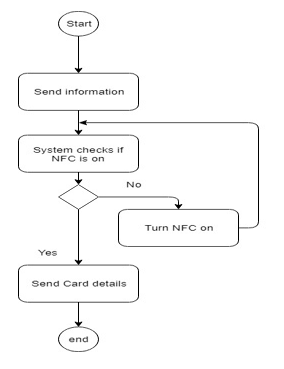
\includegraphics[width=90mm]{SystemType.PNG}
		 		\caption{An Activity diagram for sending a card.}
		 	\end{figure}
	 	
	 
	
	
	\section{Architectural Style}
	\subsection{3-Tier Architecture}
	\begin{itemize}
		\item We choose the 3-tier architectural design because we can use the model for flexibility and re usability of the application. It provides us the option to be able to modify a specific layer instead of having to redo work on the whole application.
	\end{itemize}
	\subsubsection{Presentation Layer}
		\begin{itemize}
		\item GUI - What the user sees and interacts with when our application opens.
		\end{itemize}
	
	\subsubsection{Logic Layer}
		\begin{itemize}
			\item 	The logical tier controls the application functionality by performing detailed processing.
		\end{itemize}
	\subsubsection{Database Layer}
		\begin{itemize}
			\item Store user information
			\item Store business cards	
		\end{itemize}
		
		
			\begin{figure}[ht!]
			\centering
			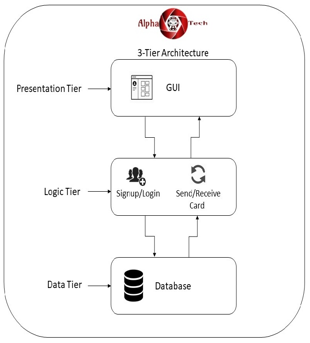
\includegraphics[width=90mm]{ArchitectureStyle.PNG}
			\caption{3-Tier Architecture design.}
		\end{figure}
	
	
	\section{Non-Functional Requirements}
	\subsection{Security}
	\begin{itemize}
		\item Authentication - Login Authentication, Single Sign On
		\item Session Management - Sessions are used to maintain state. In usual Application communication, on successful user/process Authentication, Session Identified (ID) is issued to Track authenticated state
		\item Configuration Management - Encryption(AES) to prevent unauthorized access to information.
		\item  We will use a dialog button for confirmation and cancellation	
	\end{itemize}

	\subsection{Usability}
	  \begin{itemize}
		\item Using generic interface elements(icons, fonts, menus etc) to make it simple, easy and fun to use.
		\item Utilizing the technical capabilities of the mobile device – maps, camera, phone calls, scanning etc. 
		\item It should anticipate users' needs and add value in new ways they don't expect.
		\item The visual design of the application affects the level of trust in the system and raises the degree of pleasure users get from it over time. so our look and feel need look and feel should accomplish that.
	  \end{itemize}
	\subsection{Reliability}
	Reliability test results should be stated in terms of measurements. Measurements will be taken during testing when we are collecting and analyzing data about the performance of the application.
	\begin{itemize}
		\item  An estimate of the performance of our system currently is 75% 
	\end{itemize}
	



	
\end{document}
